\documentclass[14pt,a4paper,report]{report}
\usepackage[a4paper, mag=1000, left=2.5cm, right=1cm, top=2cm, bottom=2cm, headsep=0.7cm, footskip=1cm]{geometry}
\usepackage[utf8]{inputenc}
\usepackage[english,russian]{babel}
\usepackage{indentfirst}
\usepackage[dvipsnames]{xcolor}
\usepackage[colorlinks]{hyperref}
\usepackage{listings} 
\usepackage{fancyhdr}
\usepackage{caption}
\usepackage{graphicx}
\hypersetup{
	colorlinks = true,
	linkcolor  = black
}

\usepackage{titlesec}
\titleformat{\chapter}
{\Large\bfseries} % format
{}                % label
{0pt}             % sep
{\huge}           % before-code


\DeclareCaptionFont{white}{\color{white}} 

% Listing description
\usepackage{listings} 
\DeclareCaptionFormat{listing}{\colorbox{gray}{\parbox{\textwidth}{#1#2#3}}}
\captionsetup[lstlisting]{format=listing,labelfont=white,textfont=white}
\lstset{ 
	% Listing settings
	inputencoding = utf8,			
	extendedchars = \true, 
	keepspaces = true, 			  	 % Поддержка кириллицы и пробелов в комментариях
	language = C,            	 	 % Язык программирования (для подсветки)
	basicstyle = \small\sffamily, 	 % Размер и начертание шрифта для подсветки кода
	numbers = left,               	 % Где поставить нумерацию строк (слева\справа)
	numberstyle = \tiny,          	 % Размер шрифта для номеров строк
	stepnumber = 1,               	 % Размер шага между двумя номерами строк
	numbersep = 5pt,              	 % Как далеко отстоят номера строк от подсвечиваемого кода
	backgroundcolor = \color{white}, % Цвет фона подсветки - используем \usepackage{color}
	showspaces = false,           	 % Показывать или нет пробелы специальными отступами
	showstringspaces = false,    	 % Показывать или нет пробелы в строках
	showtabs = false,           	 % Показывать или нет табуляцию в строках
	frame = single,              	 % Рисовать рамку вокруг кода
	tabsize = 2,                  	 % Размер табуляции по умолчанию равен 2 пробелам
	captionpos = t,             	 % Позиция заголовка вверху [t] или внизу [b] 
	breaklines = true,           	 % Автоматически переносить строки (да\нет)
	breakatwhitespace = false,   	 % Переносить строки только если есть пробел
	escapeinside = {\%*}{*)}      	 % Если нужно добавить комментарии в коде
}

\begin{document}

\def\contentsname{Содержание}

% Titlepage
\begin{titlepage}
	\begin{center}
		\textsc{Санкт-Петербургский Политехнический 
			Университет Петра Великого\\[5mm]
			Кафедра компьютерных систем и программных технологий}
		
		\vfill
		
		\textbf{Отчёт по лабораторной работе №7\\[3mm]
			Курс: «Операционные системы»\\[6mm]
			Тема: «Средства синхронизации потоков и процессов в ОС Windows»\\[35mm]
		}
	\end{center}
	
	\hfill
	\begin{minipage}{.5\textwidth}
		Выполнил студент:\\[2mm] 
		Бояркин Никита Сергеевич\\
		Группа: 43501/3\\[5mm]
		
		Проверил:\\[2mm] 
		Душутина Елена Владимировна
	\end{minipage}
	\vfill
	\begin{center}
		Санкт-Петербург\\ \the\year\ г.
	\end{center}
\end{titlepage}

% Contents
\tableofcontents
\clearpage

\chapter{Лабораторная работа №7}

\section{Цель работы}

Изучение средств синхронизации доступа к ресурсам потоков и процессов в ОС семейства Windows.

\section{Программа работы}

\subsubsection{Глава 1. Средства синхронизации}

\begin{enumerate}
	\item Создать два потока: производителя и потребителя. Потоки разделяют целочисленный массив, в который заносятся производимые и извлекаются потребляемые данные. Для наглядности и контроля за происходящим в буфер помещается наращиваемое значение, однозначно идентифицирующее производителя и номер его очередной посылки.
	\item Синхронизировать программу мьютексами.
	\item Синхронизировать программу семафорами.
	\item Синхронизировать программу критическими секциями.
	\item Синхронизировать программу событиями.
	\item Синхронизировать программу критическими секциями с использованием условных переменных.
\end{enumerate}


\subsubsection{Глава 2. Задача "Читатели и писатели"}

\begin{enumerate}
	\item Решить задачу одного писателя и N читателей. Для синхронизации разрешено использовать только объекты-события, в качестве разделяемого ресурса – разделяемую память (share memory). Писатель пишет в share memory сообщение и ждет, пока все читатели не прочитают данное сообщение.
	\item Решение задачи для разных процессов.
	\item Модифицировать предложенное решение таким образом, чтобы «читатели» не имели доступа к памяти по записи.
	\item Предложить более рациональное решение задачи, используя другие средства синхронизации или их сочетание.
	\item Разработать клиент-серверное приложение для полной задачи «читатели - писатели» с собственной системой ограничений на доступ каждого «читателя» к информации. Программа должна поддерживать сетевое функционирование. 
\end{enumerate}

\subsubsection{Глава 3. Задача "Обедающие философы"}

\begin{enumerate}
	\item Составить модель и программу для задачи: в одном пансионе, открытом богатым филантропом, были собраны пять знаменитых философов. Предаваясь размышлениям, они независимо друг от друга заходили обедать в общую столовую. В столовой стоял стол, вокруг которого был поставлены стулья.
	Каждому философу свой стул. Слева от философа лежало по вилке, а в центре стола стояла большая тарелка спагетти. Спагетти можно было есть только двумя вилками, а потому, сев за стол, философ должен был взять вилку соседа справа (если она, конечно, свободна).
\end{enumerate}

\clearpage

\section{Характеристики системы}

Некоторая информация об операционной системе и ресурсах системы:

\begin{figure}[h!]
	\centering
	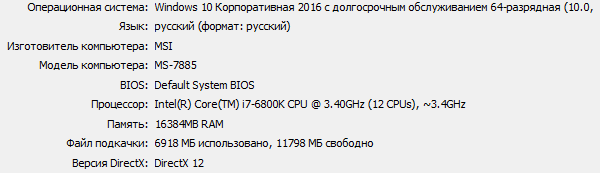
\includegraphics[scale = 1.05]{images/0.png}
	
	\caption{}
	\label{image:1}
\end{figure}

Информация о компиляторе:

\lstinputlisting{listings/0.c.log}

Информация о компоновщике:

\lstinputlisting{listings/0.l.log}

\section{Ход работы}

\subsection{Глава 1. Средства синхронизации}

В ОС Windows существует множество способов для синхронизации потоков и процессов:

\begin{enumerate}
	\item Мьютексы.
	\item Семафоры.	
	\item Критические секции.
	\item Объекты события.
	\item Условные переменные.
	\item Функции ожидания.
\end{enumerate}

Каждый из этих способов синхронизации имеет свои преимущества и недостатки.

\subsubsection{1. Создание многопоточного приложения для последующей синхронизации}

Для демонстрации работы каждого из этих средств синхронизации была написана программа, которая имеет производителя и потребителя. Потоки разделяют целочисленный массив, в который заносятся производимые и извлекаются потребляемые данные. Для наглядности и контроля за происходящим в буфер помещается наращиваемое значение, однозначно идентифицирующее производителя и номер его очередной посылки.

Главный поток определяет конфигурацию программы, создает все структуры данных и потоки. После создания всех объектов поток ожидает завершения созданных потоков, а затем производит удаление всех созданных объектов.

В программе предусматривается возможность настройки:

\begin{enumerate}
	\item Количества писателей и читателей.
	\item Установки задержек для читателей и писателей.
	\item Времени жизни приложения. 
	\item Размера очереди сообщения.
\end{enumerate}

В качестве общего ресурса используется очередь FIFO. Потоки-писатели добавляют в очередь сообщения, потоки-читатели забирают. 

Реализация программы:

\lstinputlisting{listings/p1.template.cpp}

\clearpage

Результат работы программы:

\begin{figure}[h!]
	\centering
	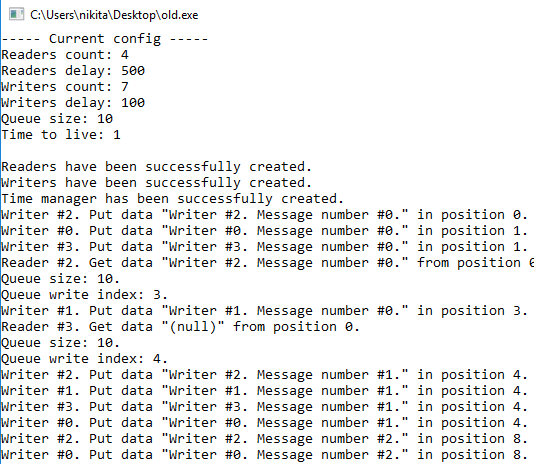
\includegraphics[scale = 0.95]{images/p1_1.png}
	
	\caption{}
	\label{image:2}
\end{figure}

Можно заметить, что результирующие данные не синхронизированны: сообщение появляются вразнобой и проскакивают значения (null). Далее, при помощи различных методов синхронизации мы постараемся избежать этой ситуации.  

\subsubsection{2. Синхронизация мьютексами}

Мьютексы гарантируют потокам взаимоисключающий доступ к единственному ресурсу. Они содержат счетчик числа пользователей, счетчик рекурсии и переменную, в которой запоминается идентификатор потока.

Мьютексы ведут себя точно так же, как и критические секции. Однако, если последние являются объектами пользовательского режима, то мьютексы являются объектами ядра. Кроме того, мьютексы позволяют синхронизировать доступ к ресурсу нескольких потоков из разных процессов. При этом можно задать максимальное время ожидания доступа к ресурсу.

Идентификатор потока определяет, какой поток захватил мьютекс, а счетчик рекурсий — сколько раз. У мьютексов много применений, и это наиболее часто используемые объекты ядра. Как правило, с их помощью защищают блок памяти, к которому обращается множество потоков. 

Мьютекс создается следующей функцией:

\begin{verbatim}
HANDLE WINAPI CreateMutex(
    _In_opt_  LPSECURITY_ATTRIBUTES  lpMutexAttributes,
    _In_      BOOL                   bInitialOwner,
    _In_opt_  LPCTSTR                lpName
);
\end{verbatim}

Для открытия мьютекса используется функция:

\begin{verbatim}
HANDLE WINAPI OpenMutex(
    _In_  DWORD    dwDesiredAccess,
    _In_  BOOL     bInheritHandle,
    _In_  LPCTSTR  lpName
);
\end{verbatim}

Для захвата ресурса используются функции семейства Wait: WaitForSingleObject, WaitForMultipleObjects и др.

\begin{verbatim}
DWORD WINAPI WaitForSingleObject(
    _In_  HANDLE  hHandle,
    _In_  DWORD   dwMilliseconds
);
\end{verbatim}

Для мьютексов сделано одно исключение в правилах перехода объектов ядра из одного состояния в другое. Допустим, поток ждет освобождения занятого объекта мьютекса. В этом случае поток обычно засыпает (переходит в состояние ожидания). Однако система проверяет, не совпадает ли идентификатор потока, пытающегося захватить мьютекс, с аналогичным идентификатором у мьютекса. Если они совпадают, система по-прежнему выделяет потоку процессорное время, хотя мьютекс все еще занят. 

Мьютекс освобождается функцией ReleaseMutex:

\begin{verbatim}
BOOL WINAPI ReleaseMutex(
    _In_ HANDLE hMutex
);
\end{verbatim}

Эта функция уменьшает счетчик рекурсии в мютексе на 1. Если данный объект передавался во владение потоку неоднократно, поток обязан вызвать ReleaseMutex столько раз, сколько необходимо для обнуления счетчика рекурсии. Как только счетчик станет равен 0, переменная, хранящая идентификатор потока, тоже обнулится, и мьютекс освободится. 

Изменения в исходной программе, для синхронизации мьютексами:

\lstinputlisting{listings/p1.2.changes.cpp}

Результат работы программы после синхронизации мьютексами при различных конфигурационных параметрах:

\begin{figure}[h!]
	\centering
	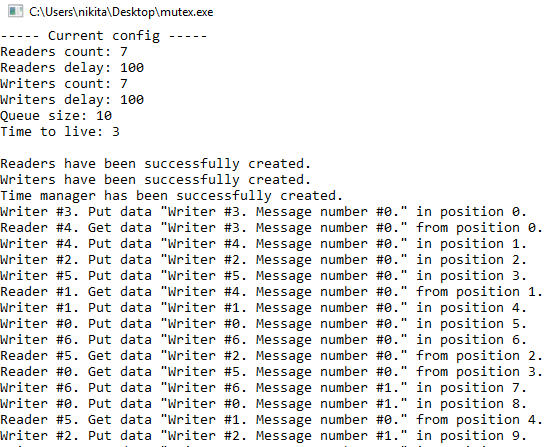
\includegraphics[scale = 0.75]{images/p1_2_1.png}
	
	\caption{}
	\label{image:3}
\end{figure}

\begin{figure}[h!]
	\centering
	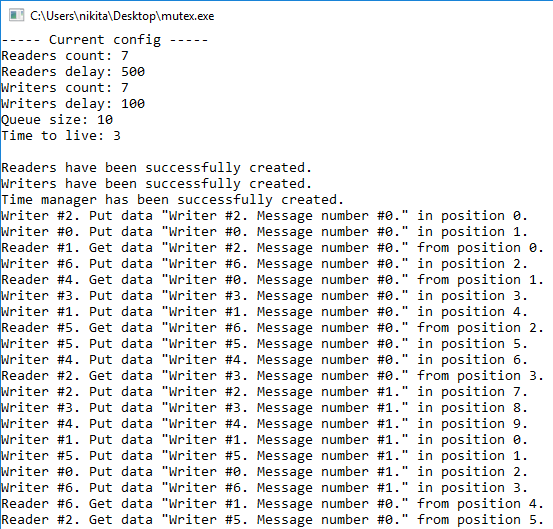
\includegraphics[scale = 0.75]{images/p1_2_2.png}
	
	\caption{}
	\label{image:4}
\end{figure}

\subsubsection{3. Синхронизация семафорами}

Семафоры используются для учета ресурсов. Как и все объекты ядра, они содержат счетчик числа пользователей, но, кроме того, поддерживают два 32 битных значения со знаком: одно определяет максимальное число ресурсов (контролируемое семафором), другое используется как счетчик текущего числа ресурсов.

Семафор создается вызовом функции CreateSemaphore:

\begin{verbatim}
HANDLE WINAPI CreateSemaphore(
    _In_opt_  LPSECURITY_ATTRIBUTES  lpSemaphoreAttributes,
    _In_      LONG                   lInitialCount,
    _In_      LONG                   lMaximumCount,
    _In_opt_  LPCTSTR                lpName
);
\end{verbatim} 

Получить существующий семафор можно с помощью функции OpenSemaphore:

\begin{verbatim}
HANDLE WINAPI OpenSemaphore(
    _In_  DWORD    dwDesiredAccess,
    _In_  BOOL     bInheritHandle,
    _In_  LPCTSTR  lpName
);
\end{verbatim} 

Для захвата ресурса используются функции семейства Wait: WaitForSingleObject, WaitForMultipleObjects и др.

Семафор освобождается функцией ReleaseSemaphore:

\begin{verbatim}
BOOL WINAPI ReleaseSemaphore(
    _In_       HANDLE  hSemaphore,
    _In_       LONG    lReleaseCount,
    _Out_opt_  LPLONG  lpPreviousCount
);
\end{verbatim} 

Изменения в исходной программе, для синхронизации семафорами:

\lstinputlisting{listings/p1.3.changes.cpp}

\clearpage

Результат работы программы после синхронизации семафорами при различных конфигурационных параметрах:

\begin{figure}[h!]
	\centering
	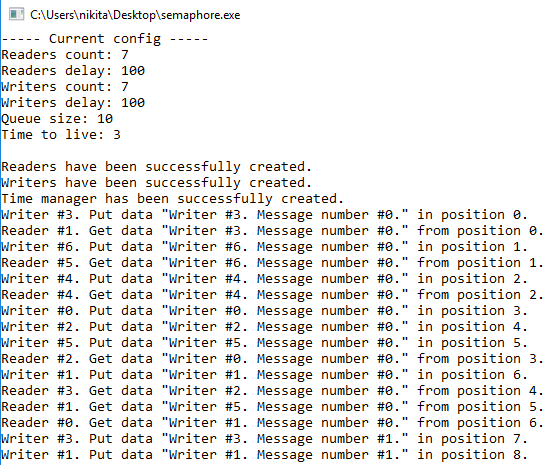
\includegraphics[scale = 0.75]{images/p1_3_1.png}
	
	\caption{}
	\label{image:5}
\end{figure}

\begin{figure}[h!]
	\centering
	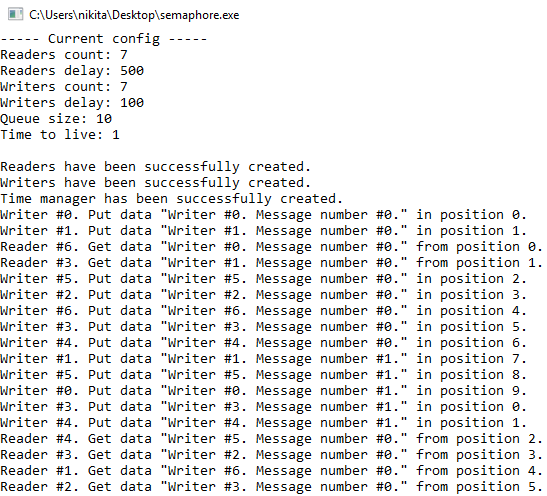
\includegraphics[scale = 0.75]{images/p1_3_2.png}
	
	\caption{}
	\label{image:6}
\end{figure}


\subsubsection{4. Синхронизация критическими секциями}

Критическая секция — небольшой участок кода, требующий монопольного доступа к каким-то общим данным. Она позволяет сделать так, чтобы единовременно только один поток получал доступ к определенному ресурсу.

Важное преимущество критической секции перед мьютексами и семафорами заключается в том, что она работает намного быстрее, ввиду того что не является объектом ядра.

Инициализация критической секции производится функцией 

\begin{verbatim}
void WINAPI InitializeCriticalSection(
    _Out_  LPCRITICAL_SECTION  lpCriticalSection
);
\end{verbatim}

Захват секции производится функцией EnterCriticalSection:

\begin{verbatim}
void WINAPI EnterCriticalSection(
    _Inout_  LPCRITICAL_SECTION  lpCriticalSection
);
\end{verbatim}

Освобождение секции производится функцией LeaveCriticalSection:

\begin{verbatim}
void WINAPI LeaveCriticalSection(
    _Inout_  LPCRITICAL_SECTION  lpCriticalSection
);
\end{verbatim}

Удаление критической секции производится функцией DeleteCriticalSection:

\begin{verbatim}
void WINAPI DeleteCriticalSection(
    _Inout_  LPCRITICAL_SECTION  lpCriticalSection
);
\end{verbatim}

Изменения в исходной программе, для синхронизации критическими секциями:

\lstinputlisting{listings/p1.4.changes.cpp}

Результат работы программы после синхронизации критическими секциями при различных конфигурационных параметрах:

\begin{figure}[h!]
	\centering
	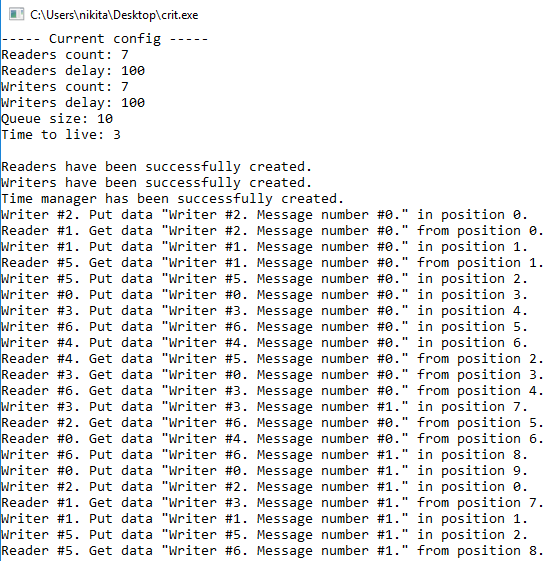
\includegraphics[scale = 0.75]{images/p1_4_1.png}
	
	\caption{}
	\label{image:7}
\end{figure}

\begin{figure}[h!]
	\centering
	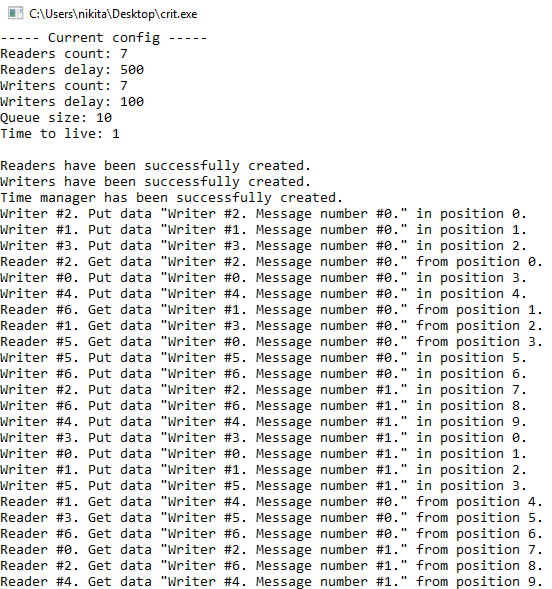
\includegraphics[scale = 0.75]{images/p1_4_2.png}
	
	\caption{}
	\label{image:8}
\end{figure}

\subsubsection{5. Синхронизация событиями}

События - самая примитивная разновидность объектов ядра. Они содержат счетчик числа пользователей (как и все объекты ядра) и две булевы переменные: одна сообщает тип данного объекта-события, другая — его состояние (свободен или занят). События просто уведомляют об окончании какой-либо операции. Объекты-события бывают двух типов: со сбросом вручную и с автосбросом. Первые позволяют возобновлять выполнение сразу нескольких ждущих потоков, вторые  только одного.

Событие создается вызовом функции CreateEvent:

\begin{verbatim}
HANDLE WINAPI CreateEvent(
    _In_opt_  LPSECURITY_ATTRIBUTES  lpEventAttributes,
    _In_      BOOL                   bManualReset,
    _In_      BOOL                   bInitialState,
    _In_opt_  LPCTSTR                lpName
);
\end{verbatim}

Для захвата ресурса используются функции семейства Wait: WaitForSingleObject, WaitForMultipleObjects и др.

Освобождение секции производится функцией SetEvent:

\begin{verbatim}
BOOL WINAPI SetEvent(
    _In_  HANDLE  hEvent
);
\end{verbatim}

Изменения в исходной программе, для синхронизации событиями:

\lstinputlisting{listings/p1.5.changes.cpp}

\clearpage

Результат работы программы после синхронизации событиями при различных конфигурационных параметрах:

\begin{figure}[h!]
	\centering
	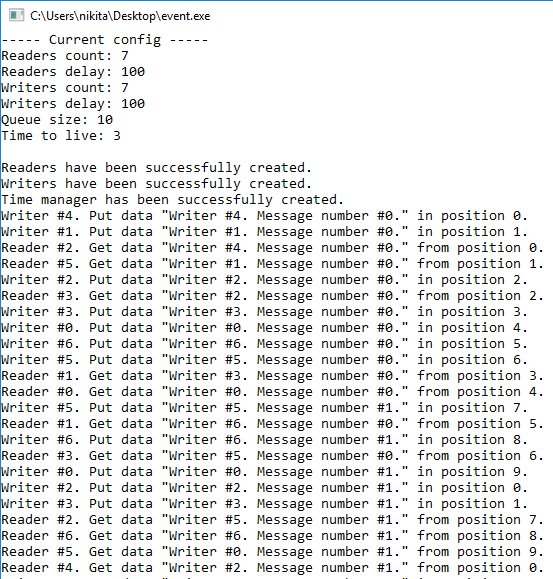
\includegraphics[scale = 0.72]{images/p1_5_1.png}
	
	\caption{}
	\label{image:9}
\end{figure}

\begin{figure}[h!]
	\centering
	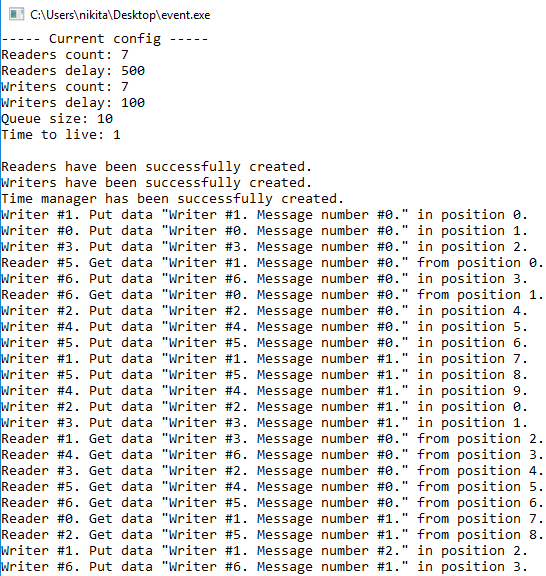
\includegraphics[scale = 0.72]{images/p1_5_2.png}
	
	\caption{}
	\label{image:10}
\end{figure}

\subsubsection{6. Синхронизация критическими секциями с использованием условных переменных}

Сами по себе условные переменные не могут применяться, а только в сочетании с другими средствами синхронизации (например, с критическими секциями). Условные переменные отсутствуют в Windows 2003 и XP. 

Инициализация условной переменной производится функцией InitializeConditionVariable:

\begin{verbatim}
VOID WINAPI InitializeConditionVariable(
    _Out_  PCONDITION_VARIABLE  ConditionVariable
);
\end{verbatim}

Для ожидания восстановления условной переменной используется функция SleepConditionVariableCS:

\begin{verbatim}
BOOL WINAPI SleepConditionVariableCS(
    _Inout_  PCONDITION_VARIABLE  ConditionVariable,
    _Inout_  PCRITICAL_SECTION    CriticalSection,
    _In_     DWORD                dwMilliseconds
);
\end{verbatim}

Для пробуждения потоков, ожидающих условной переменной используются функция:

\begin{verbatim}
VOID WINAPI WakeConditionVariable(
    _Inout_  PCONDITION_VARIABLE  ConditionVariable
);
\end{verbatim}

Изменения в исходной программе, для синхронизации критическими секциями с использованием условных переменных:

\lstinputlisting{listings/p1.6.changes.cpp}

Результат работы программы после синхронизации  критическими секциями с использованием условных переменных при различных конфигурационных параметрах:

\begin{figure}[h!]
	\centering
	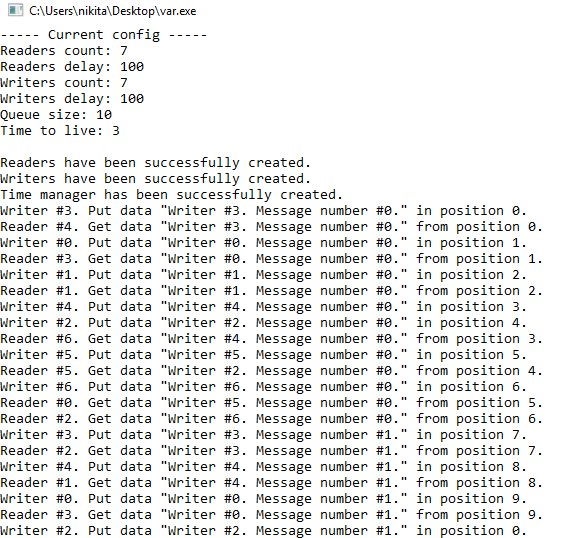
\includegraphics[scale = 0.72]{images/p1_6_1.png}
	
	\caption{}
	\label{image:11}
\end{figure}

\begin{figure}[h!]
	\centering
	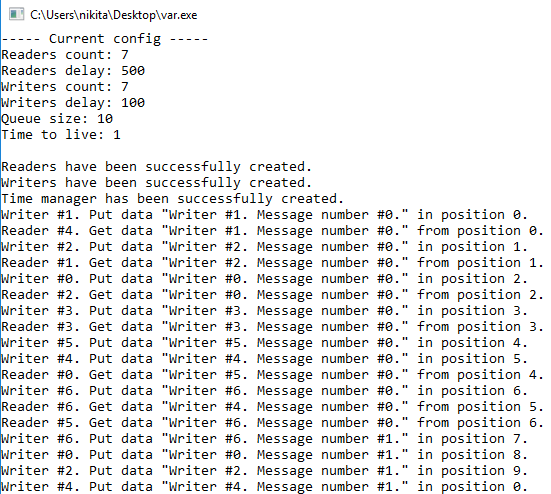
\includegraphics[scale = 0.72]{images/p1_6_2.png}
	
	\caption{}
	\label{image:12}
\end{figure}

\subsection{Глава 2. Задача <<Читатели и писатели>>}

Задача заключается в реализации одного писателя и множества читателей. Писатель пишет сообщение и ожидает пока все читатели его не прочтут.

\subsubsection{1. Использование разделяемой памяти и одного процесса для решения задачи}

Система может проецировать на оперативную память не только файл размещения, но и любой другой файл. Приложения могут использовать эту возможность. Это может использоваться для обеспечения более быстрого доступа к файлам, а также для совместного использования памяти.
 
Такие объекты называются проекциями файлов на оперативную память. Для создания проекции файла вызывается функция CreateFileMapping:

\begin{verbatim}
HANDLE WINAPI CreateFileMapping(
    _In_      HANDLE                 hFile,
    _In_opt_  LPSECURITY_ATTRIBUTES  lpAttributes,
    _In_      DWORD                  flProtect,
    _In_      DWORD                  dwMaximumSizeHigh,
    _In_      DWORD                  dwMaximumSizeLow,
    _In_opt_  LPCTSTR                lpName
);
\end{verbatim}

Для получения дескриптора уже созданного отображения используется функция OpenFileMapping:

\begin{verbatim}
HANDLE WINAPI OpenFileMapping(
 _In_  DWORD    dwDesiredAccess,
 _In_  BOOL     bInheritHandle,
 _In_  LPCTSTR  lpName
);
\end{verbatim}

Отображение файла на память процесса осуществляется с помощью функции MapViewOfFile:

\begin{verbatim}
LPVOID WINAPI MapViewOfFile(
    _In_  HANDLE  hFileMappingObject,
    _In_  DWORD   dwDesiredAccess,
    _In_  DWORD   dwFileOffsetHigh,
    _In_  DWORD   dwFileOffsetLow,
    _In_  SIZE_T  dwNumberOfBytesToMap
);
\end{verbatim}

Для очистки памяти используется функция UnmapViewOfFile:

\begin{verbatim}
BOOL WINAPI UnmapViewOfFile(
    _In_  LPCVOID  lpBaseAddress
);
\end{verbatim}

Для синхронизации потоков потребовалось пять объектов-событий:

\begin{enumerate}
	\item \emph{eventCanRead} – означает, что поток-писатель записал сообщение в память, и его могут читать потоки-читатели (ручной сброс); 

	\item \emph{eventCanWrite} – означает, что все потоки-читатели получили сообщение и готовы к приему следующего (автосброс); 

	\item \emph{eventAllRead} – требуется для приведения в готовность потоков-читателей (ручной сброс); 

	\item \emph{eventChangeCount} – событие для разрешения работы со счетчиком (количество потоков- читателей, которые прошли заданный участок кода) (автосброс); 

	\item \emph{eventExit} – устанавливается потоком-планировщиком (ручной сброс).
\end{enumerate}

Поток-писатель ждет, пока все потоки-читатели прочитают сообщение, а затем пишет новое сообщение. После записи он разрешает чтение.

\clearpage

Решение задачи <<Читатели и писатели>>:

\lstinputlisting{listings/p2.1.cpp}

\clearpage

Результат решения задачи:

\begin{figure}[h!]
	\centering
	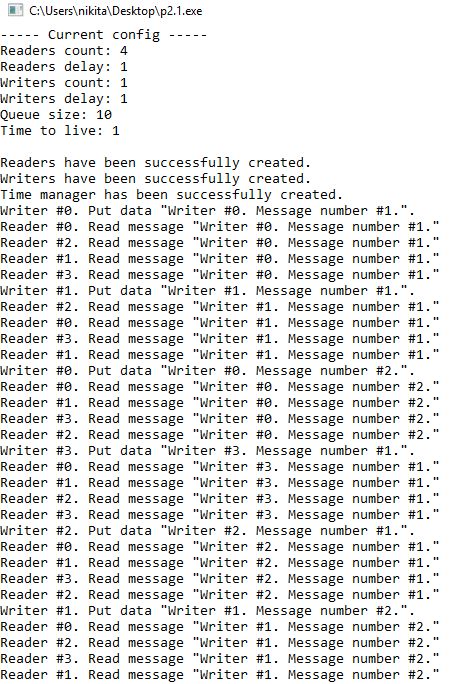
\includegraphics[scale = 0.72]{images/p2_1.png}
	
	\caption{}
	\label{image:13}
\end{figure}

После того, как писатель положил значение в разделяемую память, началось ожидание чтения всеми читателями. Только после того, как все читатели прочитали данные генерируются следующие.

\subsubsection{2. Использование разделяемой памяти и нескольких процессов для решения задачи}

В данной программе главный поток и поток-писатель будут принадлежать одному процессу, а потоки-читатели разным. Каждому событию и разделяемой памяти теперь приписывается уникальное имя, для того чтобы к ним можно было обратиться из другого процесса.

Реализация процесса-писателя:

\lstinputlisting{listings/p2.2.w.cpp}

Реализация процесса-читателя:

\lstinputlisting{listings/p2.2.r.cpp}

\clearpage

Результат работы для трех потоков писателей и трех процессов читателей:

\begin{figure}[h!]
	\centering
	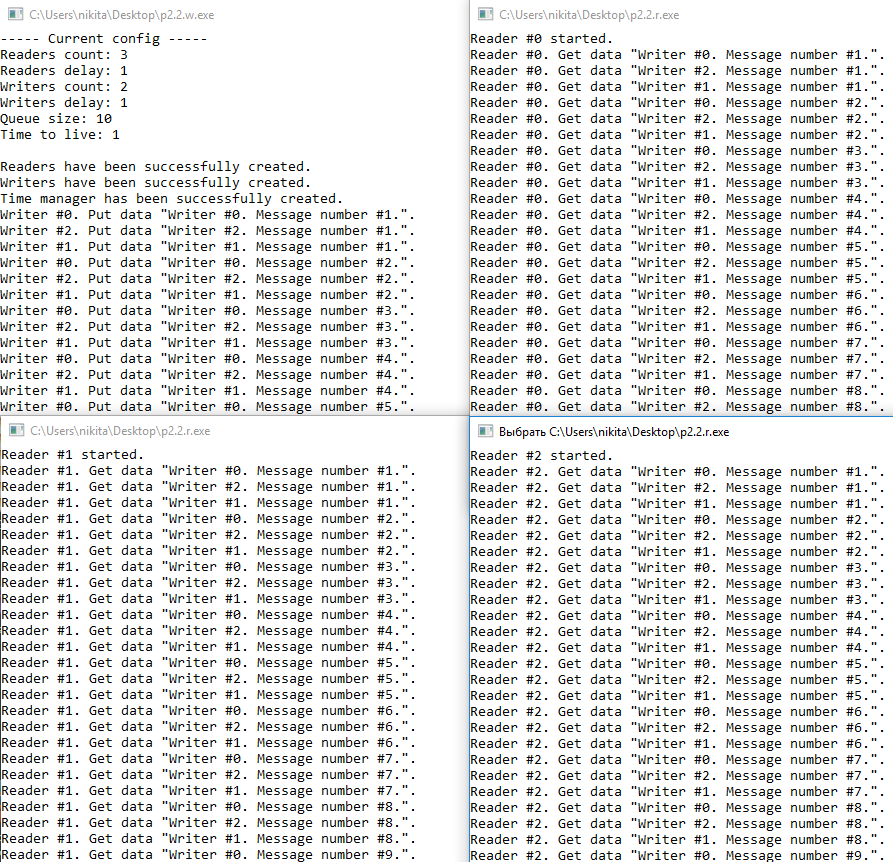
\includegraphics[scale = 0.74]{images/p2_2.png}
	
	\caption{}
	\label{image:14}
\end{figure}

Главный поток ждет завершение всех главных потоков. Т.к. потоки-читатели, принадлежащие разным процессам, имеют каждый свою консоль, то после окончания работы они сразу не завершаются, а ждут ввода любой клавиши. Каждый поток-читатель успевает читать каждое сообщение.

\subsubsection{3. Модификация программы для того, чтобы читатели не имели доступа к памяти по записи}

Для этого будем хранить счетчики в процессе писателе. Потоки-читатели вместо декремента счетчика производят освобождение событий, по которым писатель декрементирует счетчик.
 
Когда сообщение в память записано потоком-читателем, каждый читатель получает сообщение и устанавливает событие eventCount, по которому поток-писатель декрементирует значение счетчика. Когда значение этого счетчика становится равным нулю, устанавливается событие – все прочитали сообщение.

Реализация процесса-писателя:

\lstinputlisting{listings/p2.3.w.cpp}

Реализация процесса-читателя:

\lstinputlisting{listings/p2.3.r.cpp}

\clearpage

Результат работы для трех потоков писателей и трех процессов читателей:

\begin{figure}[h!]
	\centering
	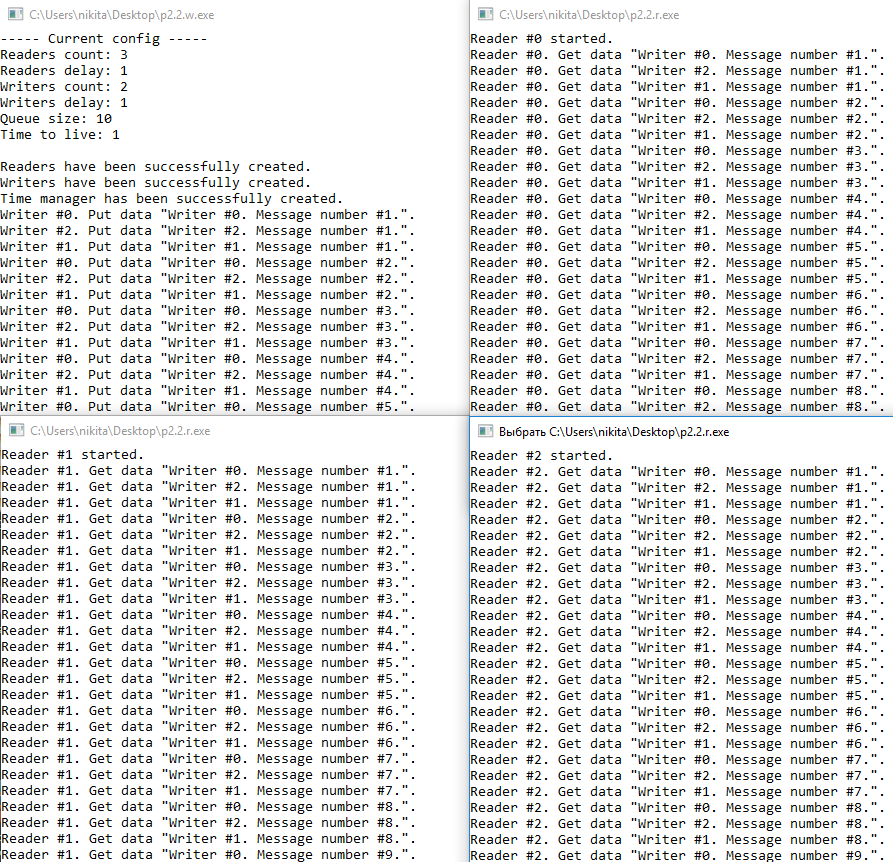
\includegraphics[scale = 0.74]{images/p2_3.png}
	
	\caption{}
	\label{image:15}
\end{figure}

Результат работы программы не изменился.  Однако теперь конструкция безопасна: читатели больше не изменяют счетчики. Счетчики расположены на стороне писателя. Общение с читателем происходит посредством событий и захватом/освобождением переменных.

\subsubsection{4. Оптимизированное решение задачи}

Используем критические секции. Они обладают высоким быстродействием по сравнению с мьютексами и, так как в данном случае мы работаем всего с одним процессом, их будет достаточно. Необходимо только синхронизировать запросы от клиентов в пределах одного процесса – сервера. Клиенты не будут подозревать о существовании других клиентов.

\lstinputlisting{listings/p2.4.rw.cpp}

Результат работы оптимизированной программы:

\begin{figure}[h!]
	\centering
	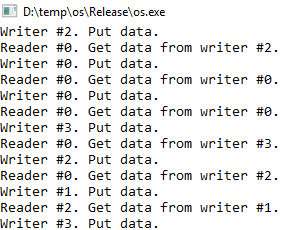
\includegraphics[scale = 0.95]{images/p2_4.png}
	
	\caption{}
	\label{image:16}
\end{figure}

\subsubsection{5. Разработка клиент-серверного приложения с сетевым функционированием}

На сервере содержится последовательно изменяющееся значение счетчика от 0 до 5. Клиент пытается угадать текущее значение счетчика. Если значение угадано, то сервер отвечает "Yes!", если не угадано, то сервер отвечает "No!".

Синхронизация доступа к переменной, которая является метафорой для любых данных, производится засчет критической секции.

Реализация серверной части:

\lstinputlisting{listings/p2.5.s.cpp}

Реализация клиентской части:

\lstinputlisting{listings/p2.5.c.cpp}

Результат отгадывания тремя клиентами одновременно:

\begin{figure}[h!]
	\centering
	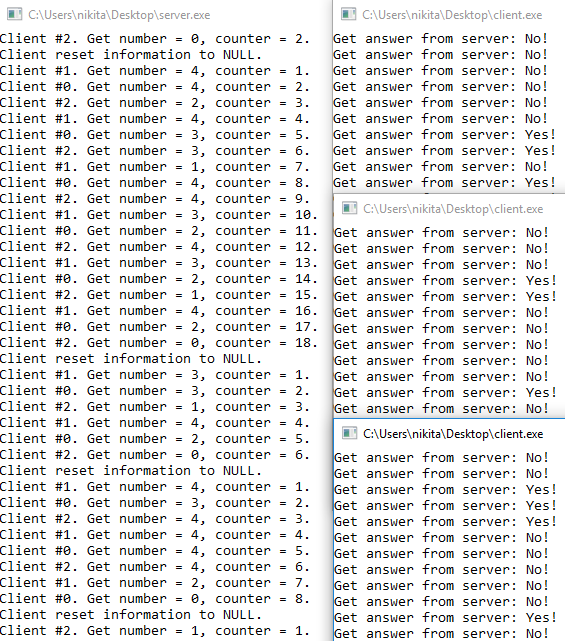
\includegraphics[scale = 0.90]{images/p2_5.png}
	
	\caption{}
	\label{image:17}
\end{figure}

\subsection{Глава 3. Задача <<Обедающие философы>>}

Формулировка задачи: в одном пансионе, открытом богатым филантропом, были собраны пять знаменитых философов. Предаваясь размышлениям, они независимо друг от друга заходили обедать в общую столовую. В столовой стоял стол, вокруг которого был поставлены стулья. Каждому философу свой стул. Слева от философа лежало по вилке, а в центре стола стояла большая тарелка спагетти. Спагетти можно было есть только двумя вилками, а потому, сев за стол, философ должен был взять вилку соседа справа (если она, конечно, свободна).

\subsubsection{1. Реализация модели и программы}

Используем мьютексы, чтобы ограничить доступ к вилкам, если они заняты другими философами. Мьютекс в данном случае – самое очевидное и элегантное решение, поскольку вилки являются метафорой для общих данных, их количество ограничено.

Для избежание дедлоков была вызывается функция std::lock в обработчике потока. Также удобно использовать функции std::bind и конструктор std::thread для передачи в обработчик потока множества аргументов. Таким образом расширенные возможности стандартной библиотеки C++ являются хорошим решением для реализации данной задачи:

\lstinputlisting{listings/p3.1.cpp}

Результат решения задачи:

\begin{figure}[h!]
	\centering
	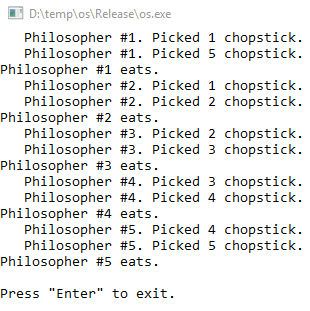
\includegraphics[scale = 0.90]{images/p3_1.png}
	
	\caption{}
	\label{image:18}
\end{figure}

Каждый филосов действительно использовал только собственную вилку и вилку соседа только в то время пока они были свободны. 

\clearpage

\section{Вывод}

В ходе работы были изучены такие средства синхронизации в ОС Windows как: семафоры, мьютексы, критические секции, объекты-события, условные переменные. Самым быстрым средством считается критическая секция, т.к. она выполняется в режиме задачи и максимально упрощена.

\begin{itemize}
	\item Мьютексы являются аналогом семафора с двумя возможными значениями. Одновременно доступ к мьютексу имеет только один поток. Мьютексы могут быть использованы для синхронизации как потоков, так и процессов.
	
	\item Семафоры позволяют захватить себя нескольким потокам, после чего захват будет невозможен, пока один из ранее захвативших семафор потоков не освободит его. Семафоры применяются для ограничения количества потоков, одновременно работающих с ресурсами. В Windows семафоры и мьютексы могут иметь имя, через которое другие процессы могут получить доступ к объектам.
	
	\item Критическая секция позволяет выделить участок кода, где поток получает доступ к разделяемому ресурсу, и предотвратить одновременное использование ресурса. К критической секции одномоментно имеет доступ только один поток. Данное средство не может быть применено для синхронизации процессов. Критическая секция не является объектом ядра, поэтому использовать функции семейства Wait не представляется возможным.
	
	\item События используются для уведомления ожидающих потоков о наступлении какого-либо события. Существует два вида событий - с ручным и автоматическим сбросом. События с ручным сбросом используются для уведомления сразу нескольких потоков. При использовании события с автоматическим сбросом уведомление получит и продолжит свое выполнение только один ожидающий поток, остальные будут ожидать дальше.
	
\end{itemize}

\section{Список литературы}

\begin{itemize}
	\item CreateMutex function [Электронный ресурс]. — URL: \href{https://msdn.microsoft.com/ru-ru/library/windows/desktop/ms682411(v=vs.85).aspx}{https://msdn.microsoft.com/ru-ru/library/windows/\linebreak desktop/ms682411(v=vs.85).aspx} (дата обращения 17.01.2017).
	
	\item CreateSemaphore function [Электронный ресурс]. — URL: \href{https://msdn.microsoft.com/ru-ru/library/windows/desktop/ms682438(v=vs.85).aspx}{https://msdn.microsoft.com/ru-ru/library/windows/\linebreak desktop/ms682438(v=vs.85).aspx} (дата обращения 17.01.2017).
	
	\item InitializeCriticalSection function [Электронный ресурс]. — URL: \href{https://msdn.microsoft.com/ru-ru/library/windows/desktop/ms683472(v=vs.85).aspx}{https://msdn.microsoft.com/ru-ru/library/\linebreak windows/desktop/ms683472(v=vs.85).aspx} (дата обращения 17.01.2017).
	
	\item CreateEvent function [Электронный ресурс]. — URL: \href{https://msdn.microsoft.com/ru-ru/library/windows/desktop/ms682396(v=vs.85).aspx}{https://msdn.microsoft.com/ru-ru/library/windows/\linebreak desktop/ms682396(v=vs.85).aspx} (дата обращения 17.01.2017).
	
	\item CreateEvent function [Электронный ресурс]. — URL: \href{https://msdn.microsoft.com/ru-ru/library/windows/desktop/ms682396(v=vs.85).aspx}{https://msdn.microsoft.com/ru-ru/library/windows/\linebreak desktop/ms682396(v=vs.85).aspx} (дата обращения 17.01.2017).
	
	\item InitializeConditionVariable function [Электронный ресурс]. — URL: \href{https://msdn.microsoft.com/ru-ru/library/windows/desktop/ms683469(v=vs.85).aspx}{https://msdn.microsoft.com/ru-ru/library/\linebreak windows/desktop/ms683469(v=vs.85).aspx} (дата обращения 17.01.2017).
	
	\item CreateFileMapping function [Электронный ресурс]. — URL: \href{https://msdn.microsoft.com/ru-ru/library/windows/desktop/aa366537(v=vs.85).aspx}{https://msdn.microsoft.com/ru-ru/library/windows/\linebreak desktop/aa366537(v=vs.85).aspx} (дата обращения 17.01.2017).
	
	\item Взаимодействие между процессами [Электронный ресурс]. — URL: \href{http://www.cyberguru.ru/win32/windows-processes-page14.html}{http://www.cyberguru.ru/win32/\linebreak windows-processes-page14.html} (дата обращения 17.01.2017).
\end{itemize}

\end{document}